\documentclass[12pt]{article}

\usepackage{sbc-template}

%Image-related packages
\usepackage{graphicx}
\usepackage{subcaption}
\usepackage[utf8]{inputenc}
\usepackage[export]{adjustbox}
\usepackage{wrapfig}
%------------------------------
\usepackage[brazil]{babel}   
%\usepackage[latin1]{inputenc}  
\usepackage[utf8]{inputenc}  
% UTF-8 encoding is recommended by ShareLaTex
\usepackage{graphicx}
     
\sloppy
\title{Protótipo do Sistema Pequira}

\author{Ariel R. Nessi\inst{1}, Cristian Cotrena\inst{1}, Matheus S. Redecker\inst{1} }


\address{Pontifícia Universidade Católica do Rio Grande do Sul - PUCRS}

\begin{document} 

\maketitle

\section{Descrição do Sistema}
O sistema Pequira tem o objetivo de ajudar os pacientes com transtornos de ansiedade possibilitando um acompanhamento em casa ou no próprio consultório com tarefas propostas pelo médico. O sistema possui duas interfaces, uma para cada usuário, médico e paciente. Com a disseminação de dispositivos móveis como tablets e smartphones o grupo decidiu se aproveitar ao máximo de padrões visuais encontrados em aplicativos para celulares, com o objetivo de trazer uma interface familiar mesmo a um grupo que não possui por hábito a utilização de um computador. Neste trabalho primeiro iremos abordar a interface do médico, explicando os padrões utilizados e o fluxo de navegação, então apresentaremos a interação do paciente com o sistema.

\section{Protótipo}
A tela inicial do sistema consiste um simples login, conforme a Figura \ref{login} o usuário e senha do sistema são registrados durante a instalação do programa, em caso de perda de senha o médico deve entrar em contato com a central de atendimento, dessa maneira uma camada de segurança adicional é inserida no sistema.

\begin{figure}[h]
\centering
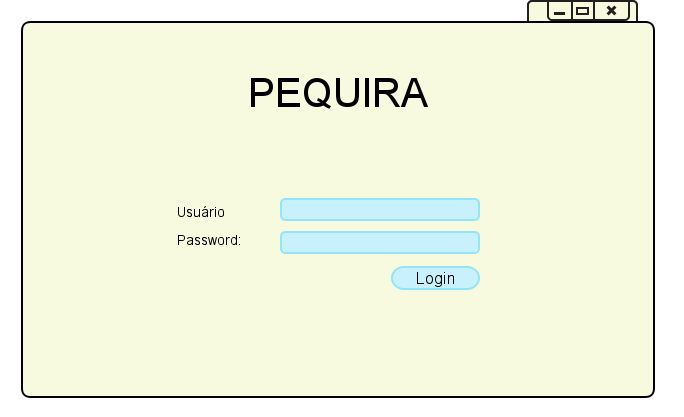
\includegraphics[scale=0.4]{imagens/1Log_In.jpg}
\caption{login}
\label{login}
\end{figure}

Esta imagem estabelece alguns padrões do sistema, a cor azul é utilizada para sinalizar um formulário, bem como a cor de fundo neutra. Após efetuar o login o médico se depara com 3 possiveis telas diferentes. A funcionalidade básica desta tela consiste em buscar e cadastrar pacientes no sistema, na Figura \ref{menu_sem_pendrive} é possivel ver estas opções, exibidas como ícones, aqui utilizamos a forma de usuário utilizada pelo facebook aliada a simbolos bem estabelecidos em diversos sistemas.

\begin{figure}[h]
\centering
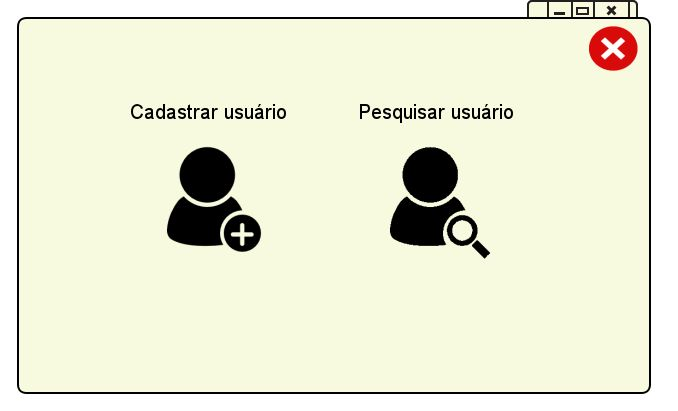
\includegraphics[scale=0.6]{imagens/1-2Usuarios_Sem_Pendrive.jpg}
\caption{Menu Inicial}
\label{menu_sem_pendrive}
\end{figure}

Nas telas seguintes uma opção adicional é exibida com a identificação de um pendrive na máquina. Caso o pendrive esteja formatado uma opção de instalar é exibida, conforme Figura \ref{menu_com_pendrive1}, caso o pendrive inserido contenha dados de um paciente uma opção para acessar diretamente o cadastro do mesmo é exibida, conforme imagem \ref{menu_com_pendrive2}.
\begin{figure}[h]
\begin{subfigure}{0.5\textwidth}
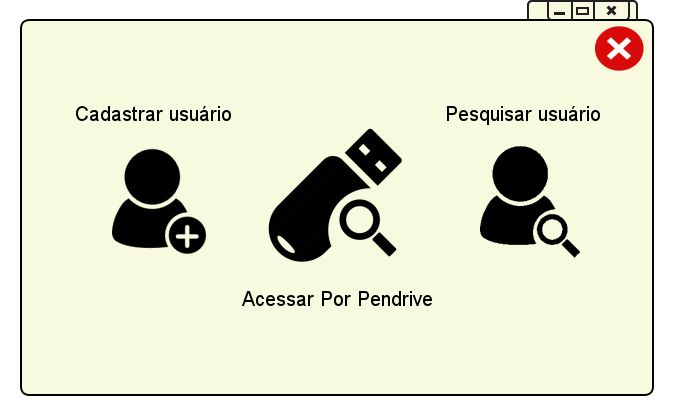
\includegraphics[scale=0.3]{imagens/1-1Usuarios_Com_Pendrive.jpg}
\caption{Acessar cadastro por pendrive}
\label{menu_com_pendrive1}
\end{subfigure}
\begin{subfigure}{0.5\textwidth}
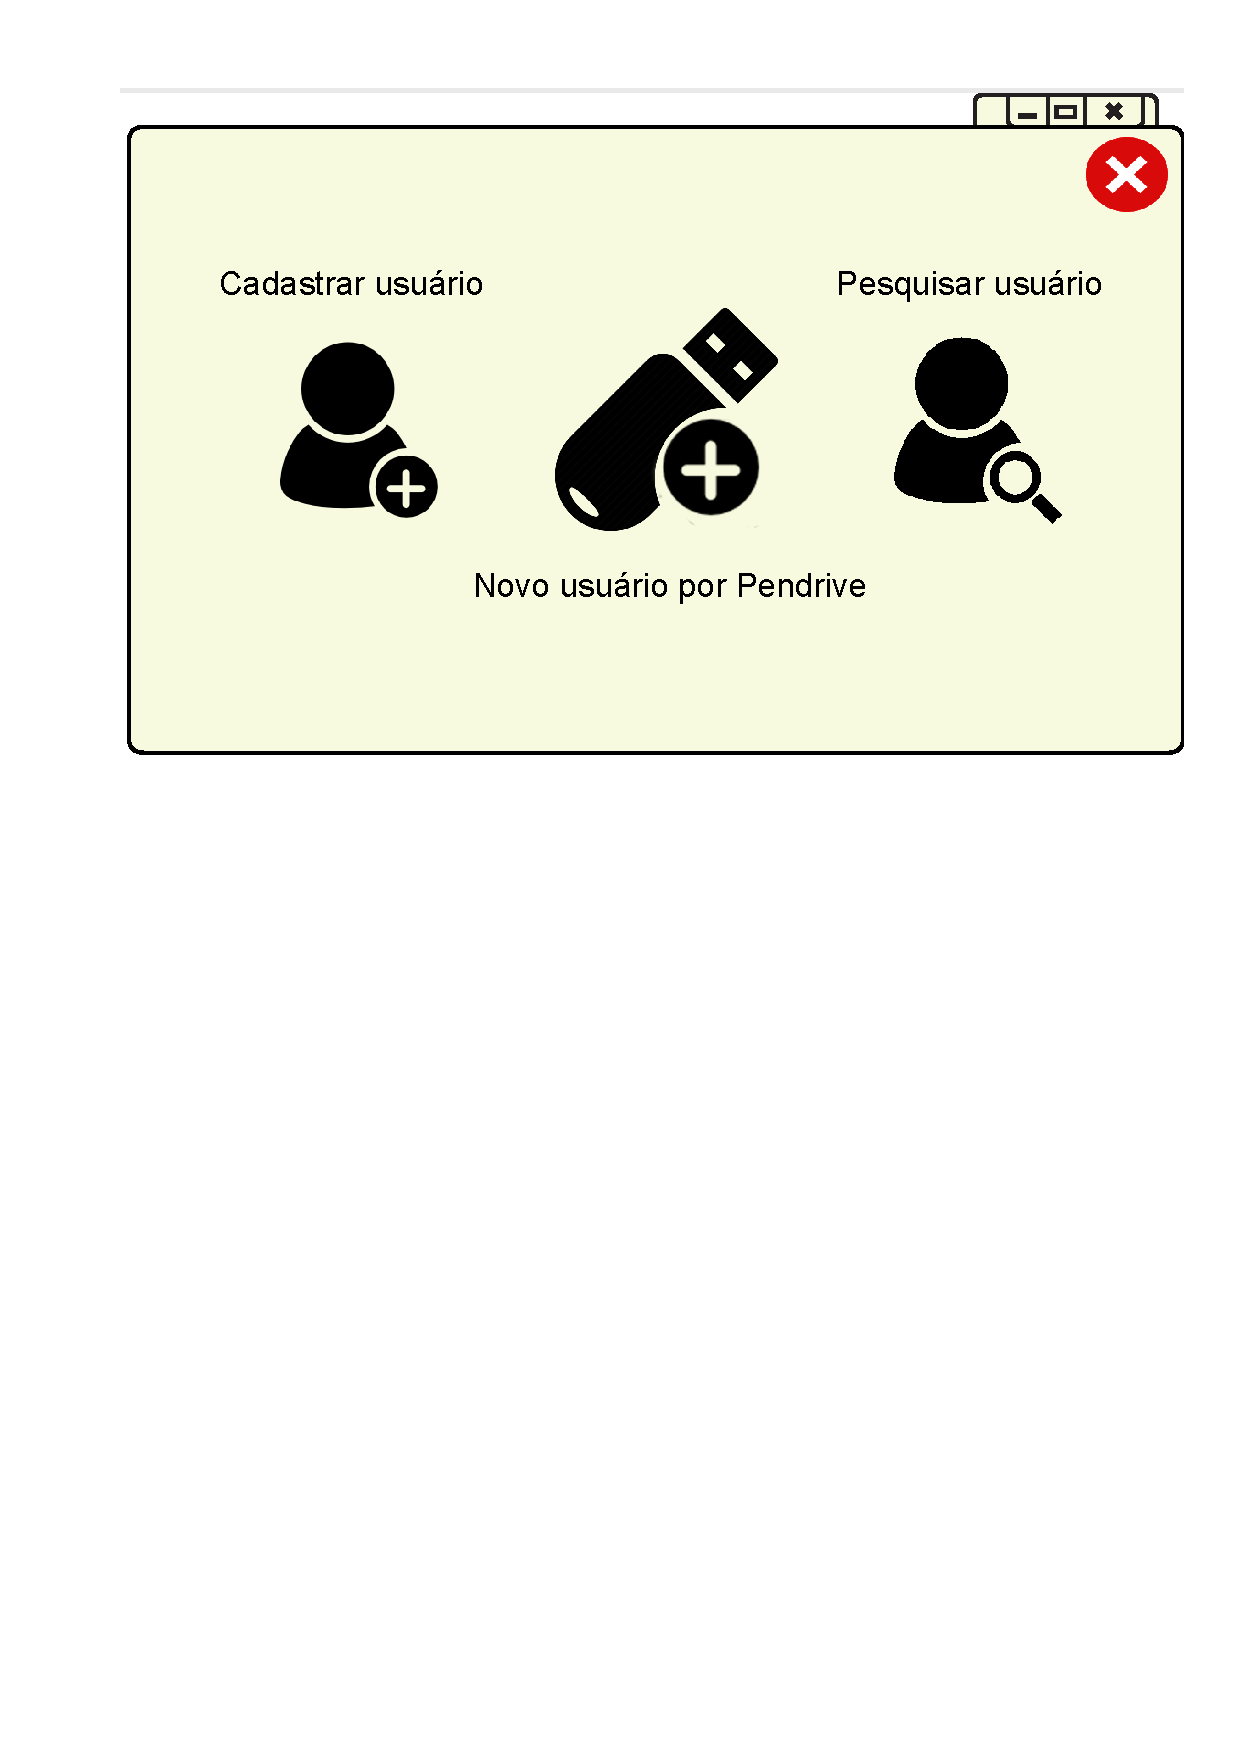
\includegraphics[scale=0.3]{imagens/1-3ProjetoInterface_1-3UsuaioComPendriveVazio.pdf} 
\caption{Novo usuário com pendrive}
\label{menu_com_pendrive2}
\end{subfigure}
\end{figure}
\newpage
Através da opção "Pesquisar Usuário" uma tela surge com campos de pesquisa como na Figura \ref{busca_usuario}, caso mais de um registro seja retornado pela pesquisa o médico deve escolher de uma lista como ilustrado na imagem \ref{busca_usuario1}.

\begin{figure}[h]
\begin{subfigure}{0.5\textwidth}
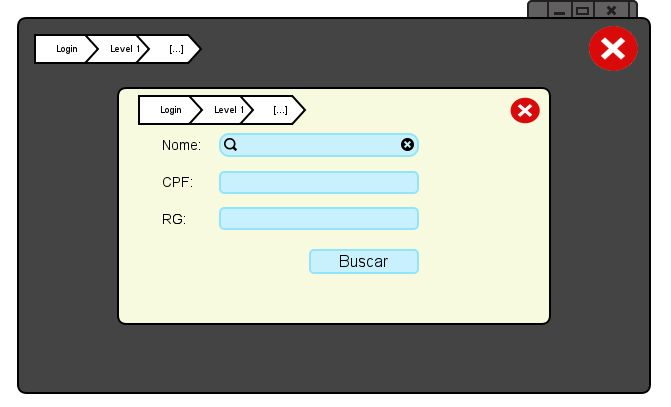
\includegraphics[scale=0.3]{imagens/1-1Buscar_Usuario.jpg}
\caption{Busca de usuários}
\label{busca_usuario}
\end{subfigure}
\begin{subfigure}{0.5\textwidth}
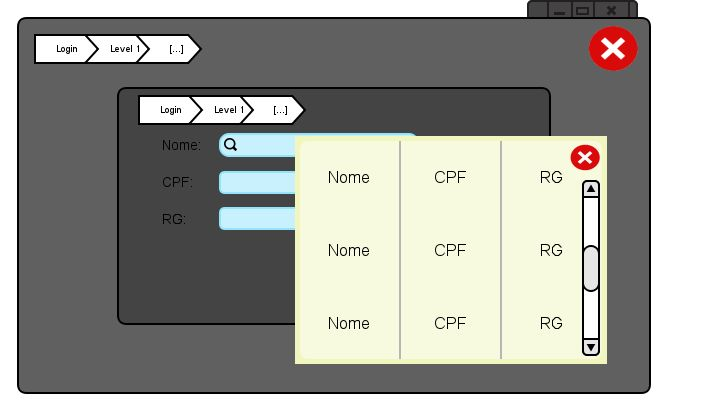
\includegraphics[scale=0.3]{imagens/1-1Multiplos_Resultados.jpg} 
\caption{Lista de usuarios}
\label{busca_usuario1}
\end{subfigure}
\end{figure}

Vale notar também nas telas que o sistema conta com breadcrumbs, facilitando assim a navegação do médico. Assim que um paciente é escolhido o nome completo do paciente é adicionado ao breadcrumb, a tela do paciente consiste em duas opções principais conforme a Figura \ref{2Tela_Usuario}, uma mensagem de erro é exibida caso o pendrive do paciente não esteja inserido, bloqueando a opção de configurar o pendrive.
\newpage
\begin{figure}[h]
\begin{subfigure}{0.5\textwidth}
\centering
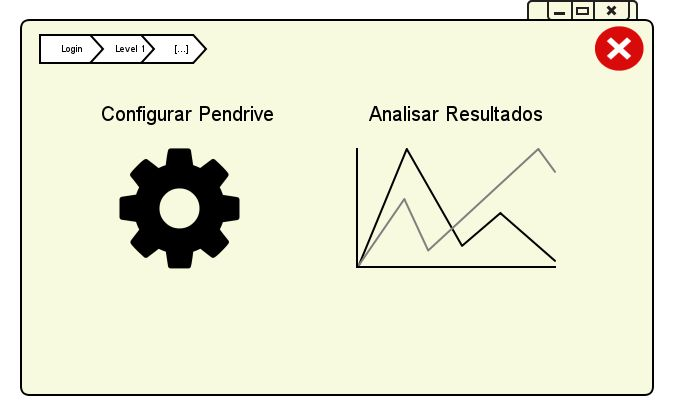
\includegraphics[scale=0.3]{imagens/2Tela_Usuario.jpg}
\caption{Tela do paciente}
\label{2Tela_Usuario}
\end{subfigure}
\begin{subfigure}{0.5\textwidth}
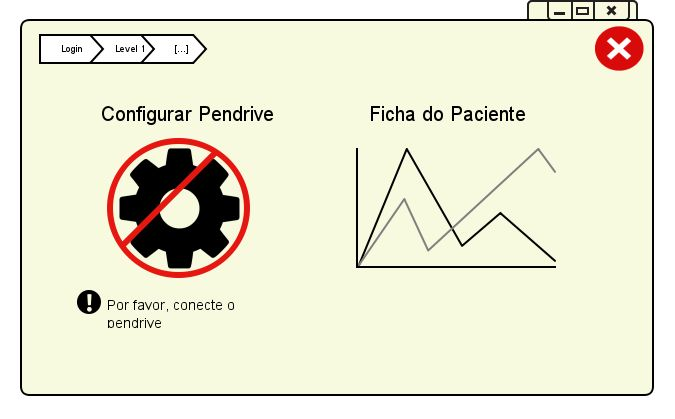
\includegraphics[scale=0.3]{imagens/2-1Tela_Usuario_Sem_Pednrive.jpg} 
\caption{Tela do paciente sem pendrive}
\label{2Tela_Usuario1}
\end{subfigure}
\end{figure}

Nesta tela o padrão de usar icones é mantido, contudo ao interagir com um dos icones a transição para uma nova tela não é imediata, uma variação do padrão overlay menu é aplicada, trazendo um menu diferente para cada icone como nas figuras \ref{configurar_pendrive} e \ref{ficha_do_paciente}.

\begin{figure}[h]
\begin{subfigure}{0.5\textwidth}
\centering
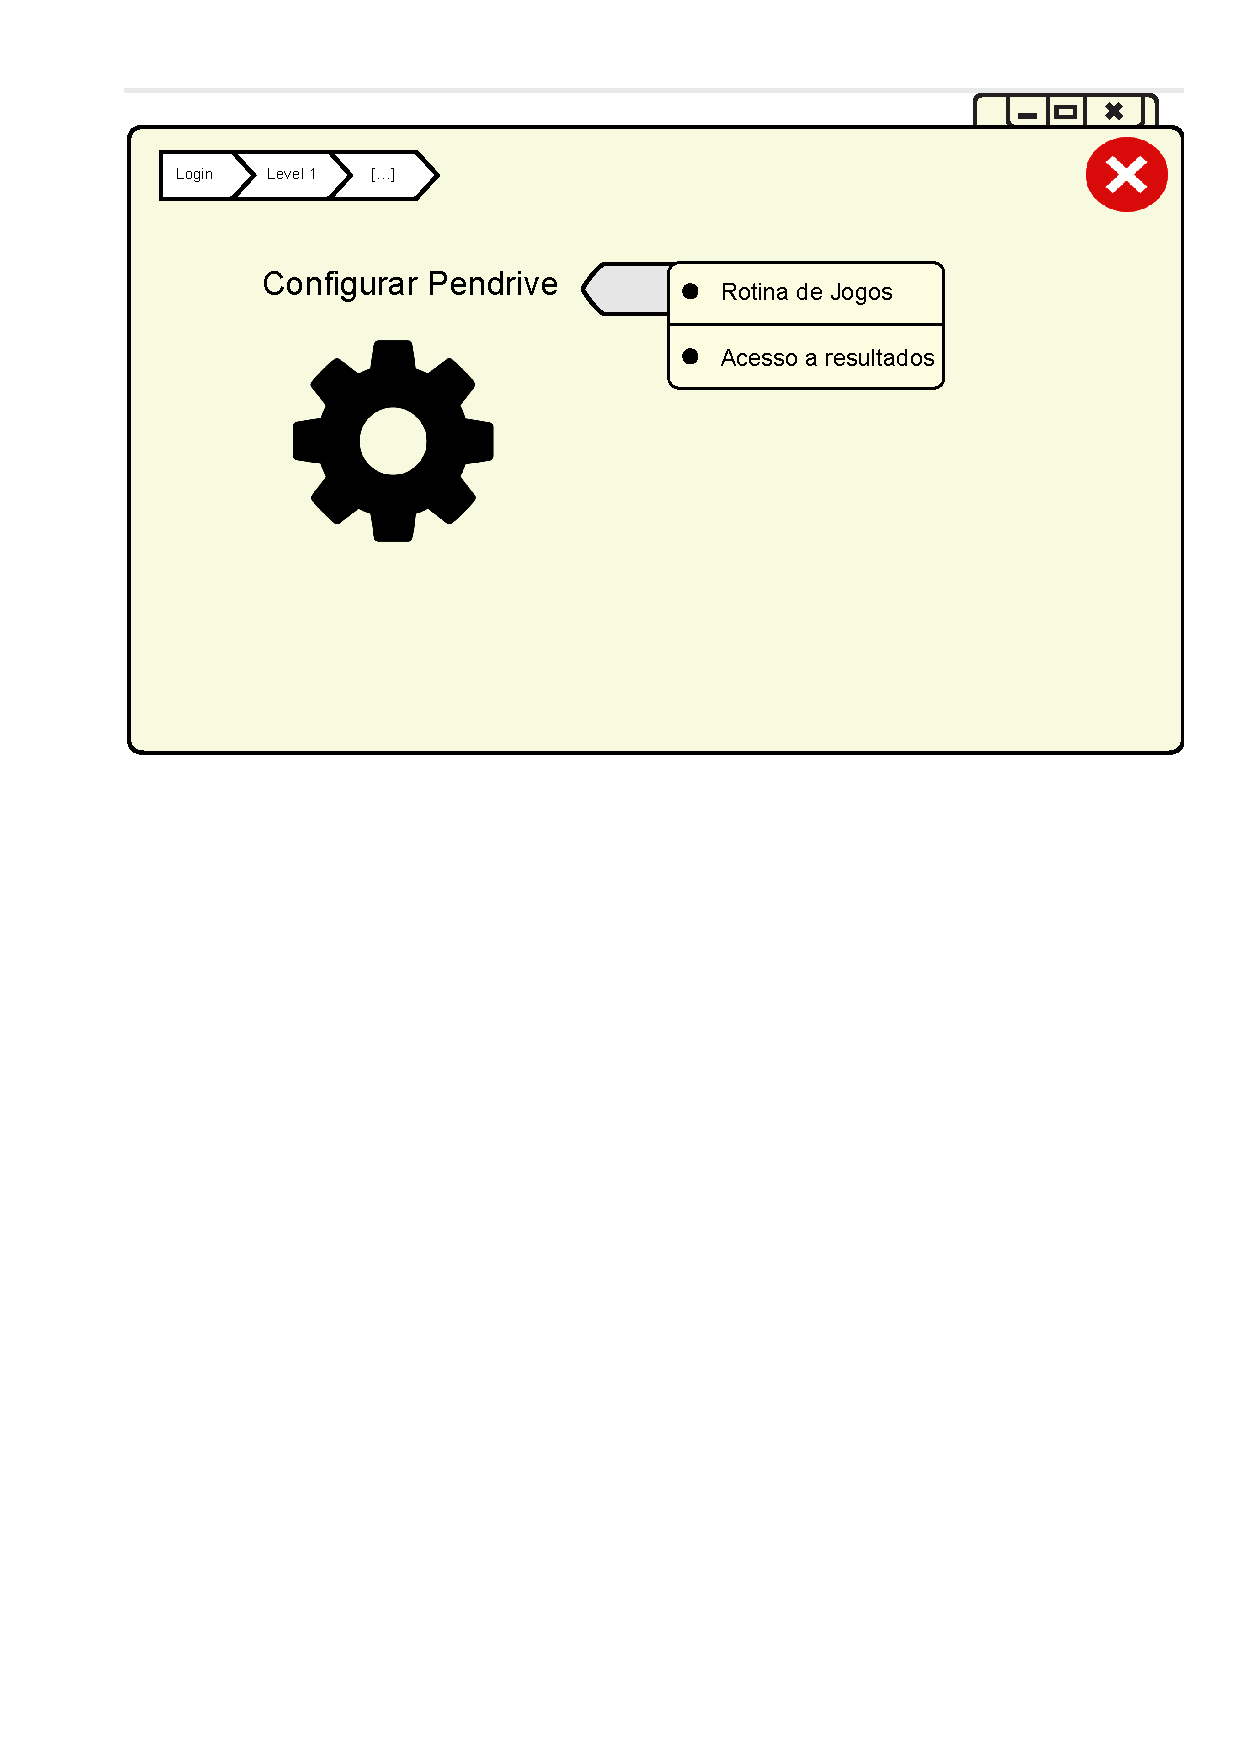
\includegraphics[scale=0.3]{imagens/2-4Configurar_Pendrive_Menu.pdf}
\caption{Menu Configurar Pendrive}
\label{configurar_pendrive}
\end{subfigure}
\begin{subfigure}{0.5\textwidth}
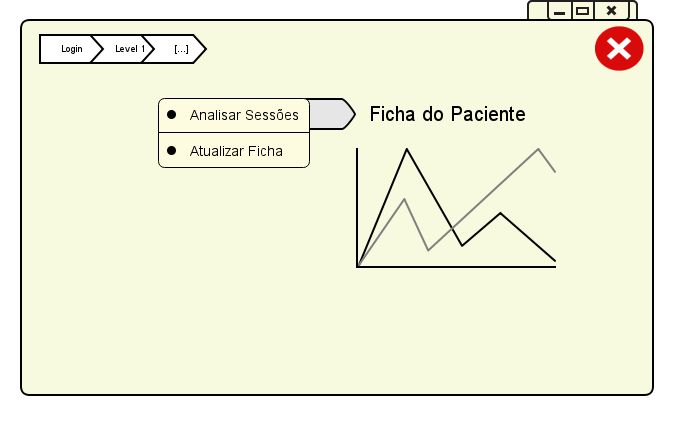
\includegraphics[scale=0.3]{imagens/2-3Ficha_do_Paciente_Menu.jpg} 
\caption{Menu Ficha do Paciente}
\label{ficha_do_paciente}
\end{subfigure}
\end{figure}

Ao selecionar a opção "Rotina de Jogos" da Figura \ref{configurar_pendrive} um wizard é iniciado, os passos deste wizard servem para definir os períodos em que o paciente pode acessar o sistema, por quanto tempo, quais jogos e em que período a configuração é valida.
\newpage
\begin{figure}[h]
\centering
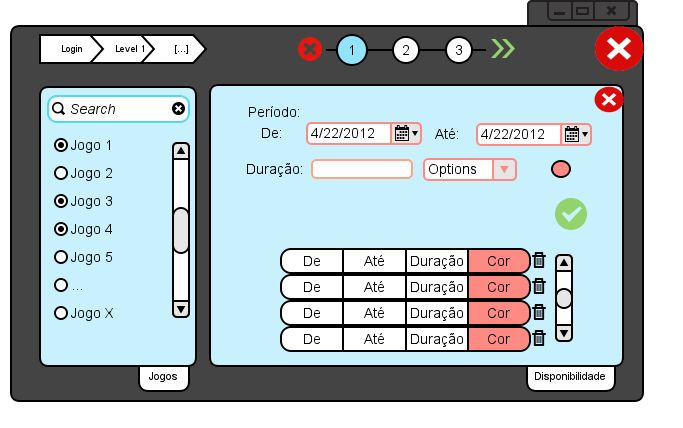
\includegraphics[scale=0.6]{imagens/2-4-1-1Configurar_Pendrive_Rotina_1.jpg}
\caption{Wizard de configuração, 1º Passo}
\label{wizard1}
\end{figure}

Na figura \ref{wizard1} tela é dividida em duas áreas diferentes, "Jogos" e "Disponibilidade", na primeira o médico deve escolher os jogos que estarão disponíves, uma caixa de busca é disponibilizada para auxiliar na busca dos mesmos. Na segunda tela um conjunto de legendas podem ser adicionadas, removidas e alteradas. A borda das caixas de texto desta janela são coloridas conforme a cor escolhida para a legenda.

\begin{figure}[h!]
\centering
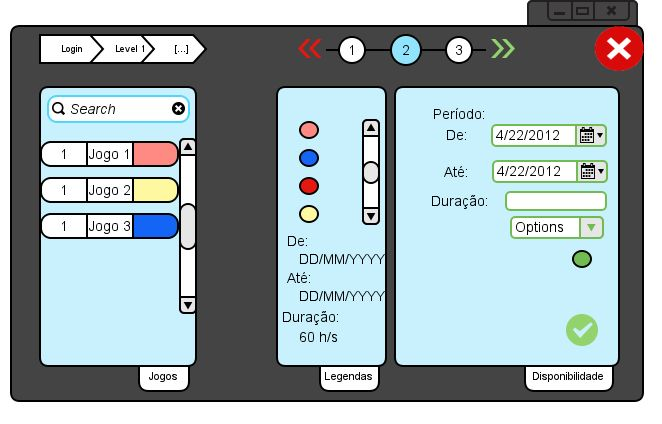
\includegraphics[scale=0.6]{imagens/2-4-1-2Configurar_Pendrive_Rotina_2.jpg}
\caption{Wizard de configuração, 2º Passo}
\label{wizard2}
\end{figure}

O médico navega entre os passos do wizard através das setas ou do número do passo, localizados ao centro no topo da tela. No segundo passo do wizard o médico deve ordenar em que sequencia os jogos selecionados devem ser jogados pelo paciente, bem como associar cada jogo à uma legenda de disponibilidade, a tela é agora quebrada em três, a divisão "Legendas" traz as configurações de disponibilidade que já foram adicionadas, ao passar com o mouse sobre uma das cores informações sobre esta legenda é apresentada.
\begin{figure}[h]
\centering
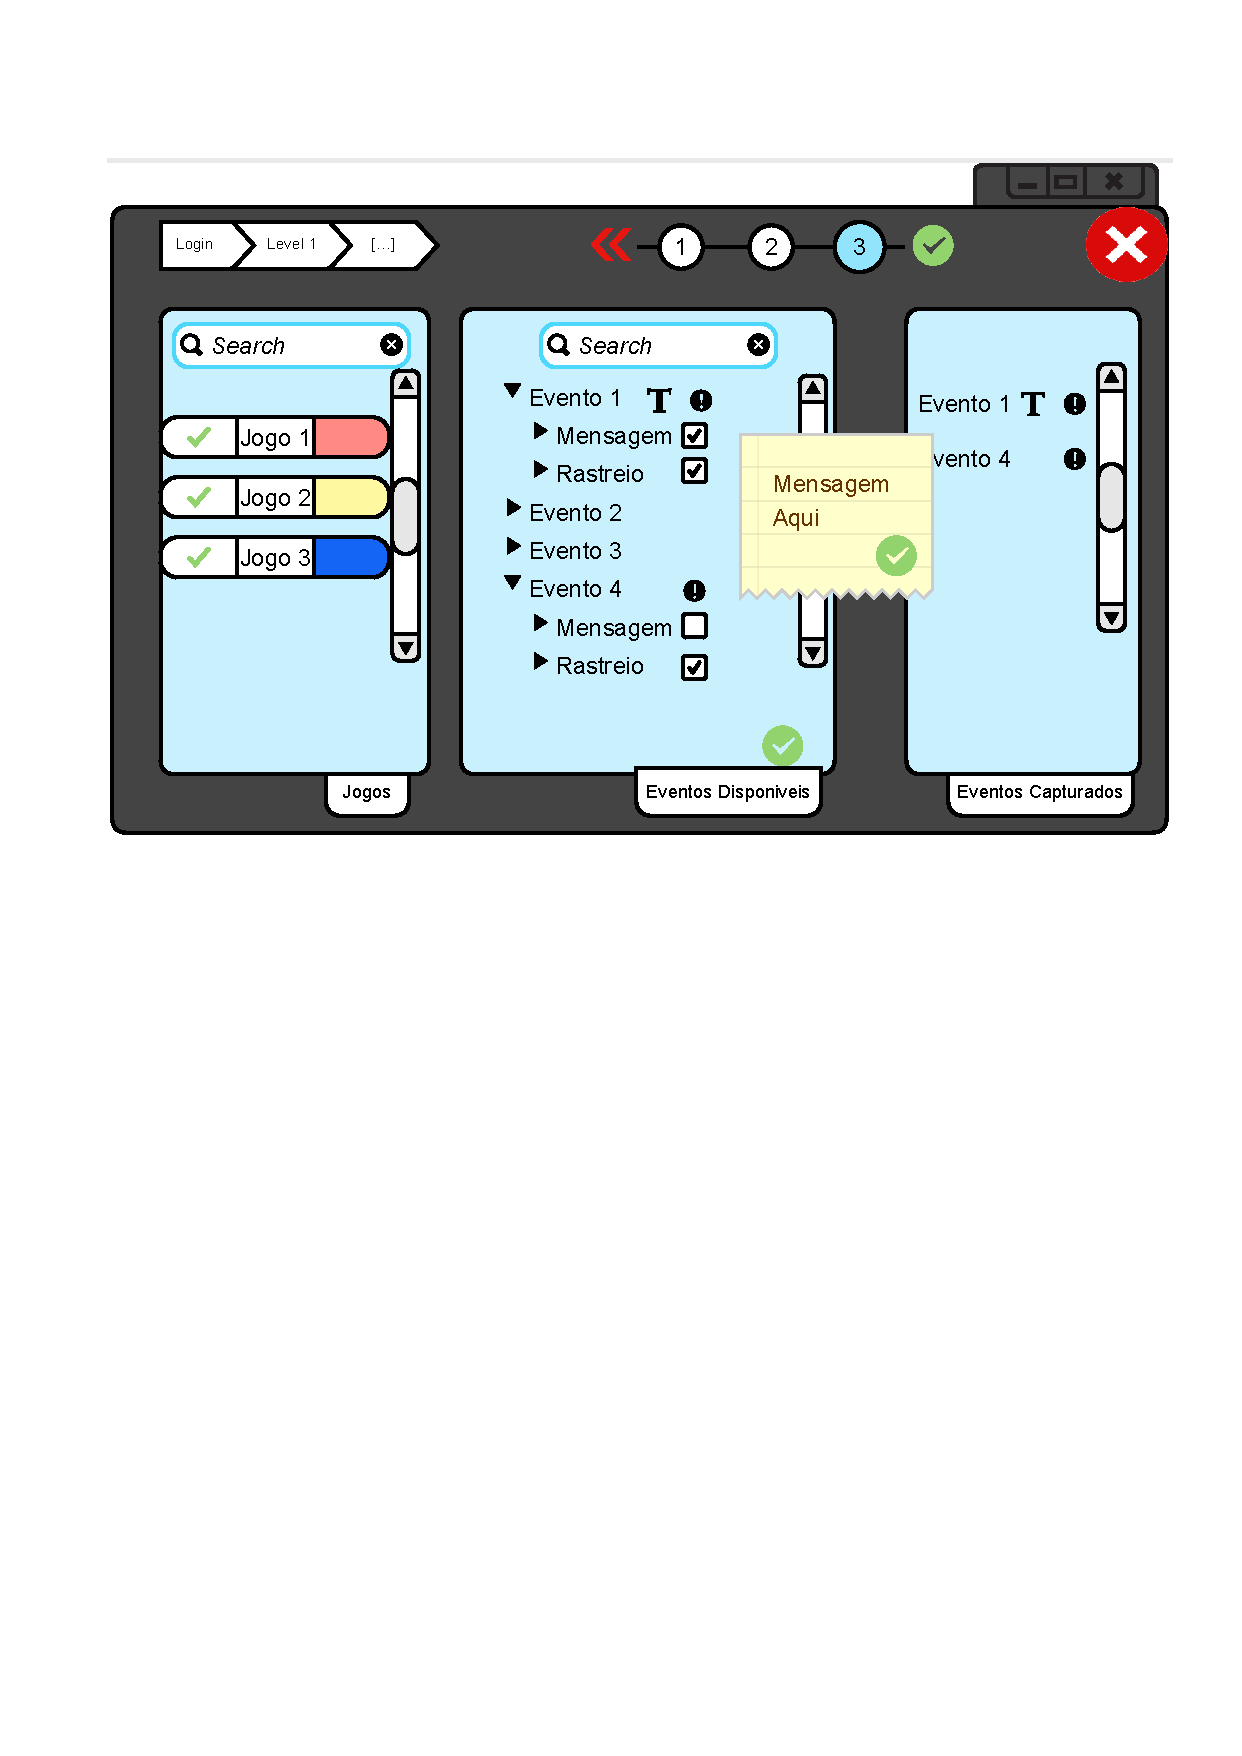
\includegraphics[scale=0.6]{imagens/2-4-1-3Configurar_Pendrive_Rotina_3.pdf}
\label{wizard3}
\caption{Wizard de configuração, 3º Passo}
\end{figure}

No último passo do wizard o médico pode selecionar eventos para rastrear ou disparar mensagens motivacionais. A última coluna serve para visualizar os eventos habilitados para cada jogo. Para habilitar o mesmo evento para diversos jogos basta selecionar um conjunto de jogos e então marcar os eventos desejados. Dois ícones são introduzidos nesta tela, um sinal de exclamação simboliza eventos com a função de rastreio habilitada, enquanto o \textbf{T} simboliza a função de mensagem para um evento. Na figura \ref{wizard3} um exemplo de preenchimento do terceiro passo é fornecido.
\newpage
Voltando ainda ao menu da Figura \ref{configurar_pendrive} ao acessar a opção "Acesso a resultados" o médico é levado à uma tela com as sessões registradas, o médico pode avaliar as sessões e permitir que o paciente visualize seus resultados. A opção "Analisar Sessões" na Figura \ref{ficha_do_paciente} leva à mesma tela, demonstrada na Figura \ref{analisar_sessoes}.

\begin{figure}[h]
\centering
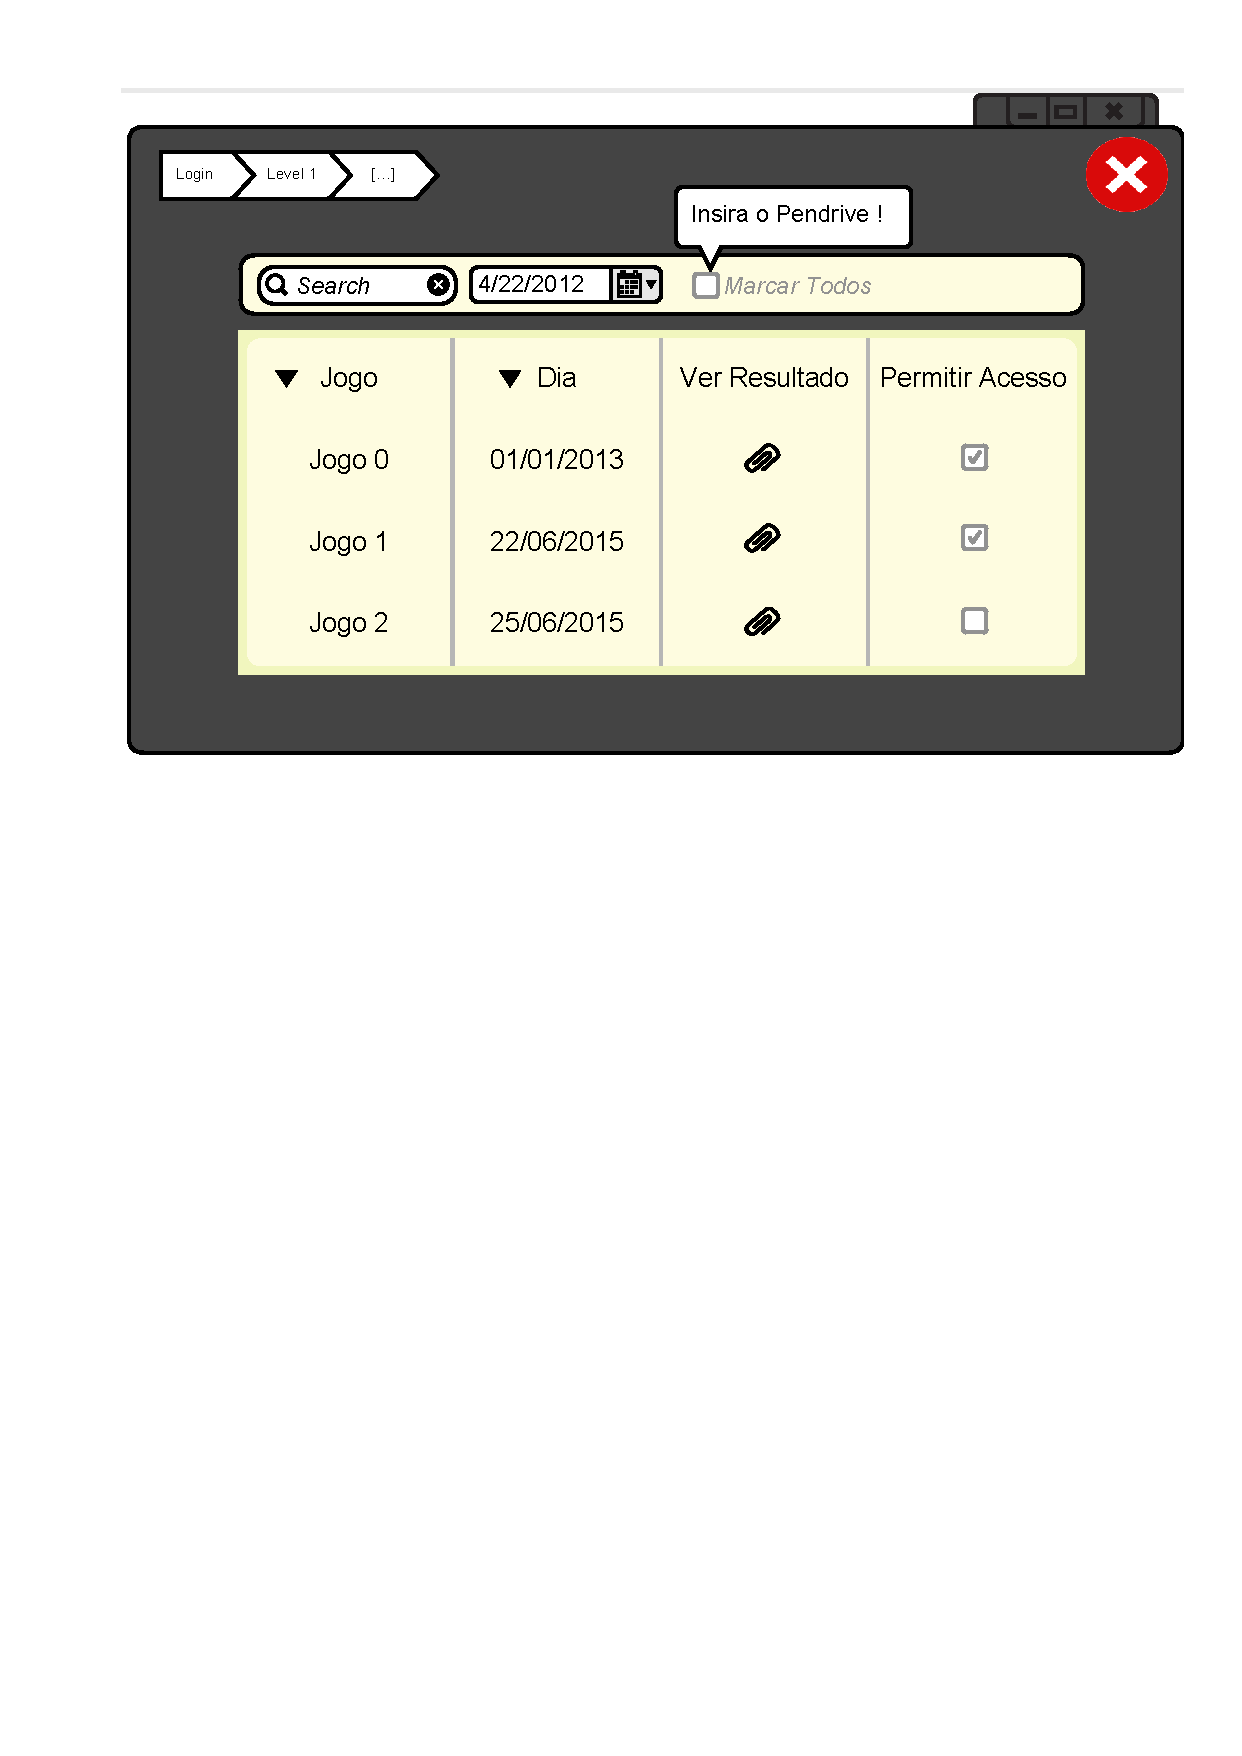
\includegraphics[scale=0.6]{imagens/2-4-2-1Acesso_resultados.pdf}
\label{analisar_sessoes}
\caption{Lista de sessões salvas}
\end{figure}

Ao selecionar uma das sessões e clicar no ícone de anexo uma nova tela abre com os sinais do emotiv e um video frontal do usuário. Nesta tela o médico pode selecionar as ondas que deseja analisar e os eventos que devem estar sinalizados na linha do emotiv, na Figura \ref{emotiv} podemos ver a linha do emotiv na area superior, com algumas marcações de eventos pela linha, na Figura \ref{emotiv1} as opções do menu lateral são expostas. 

\begin{figure}[h]
\centering
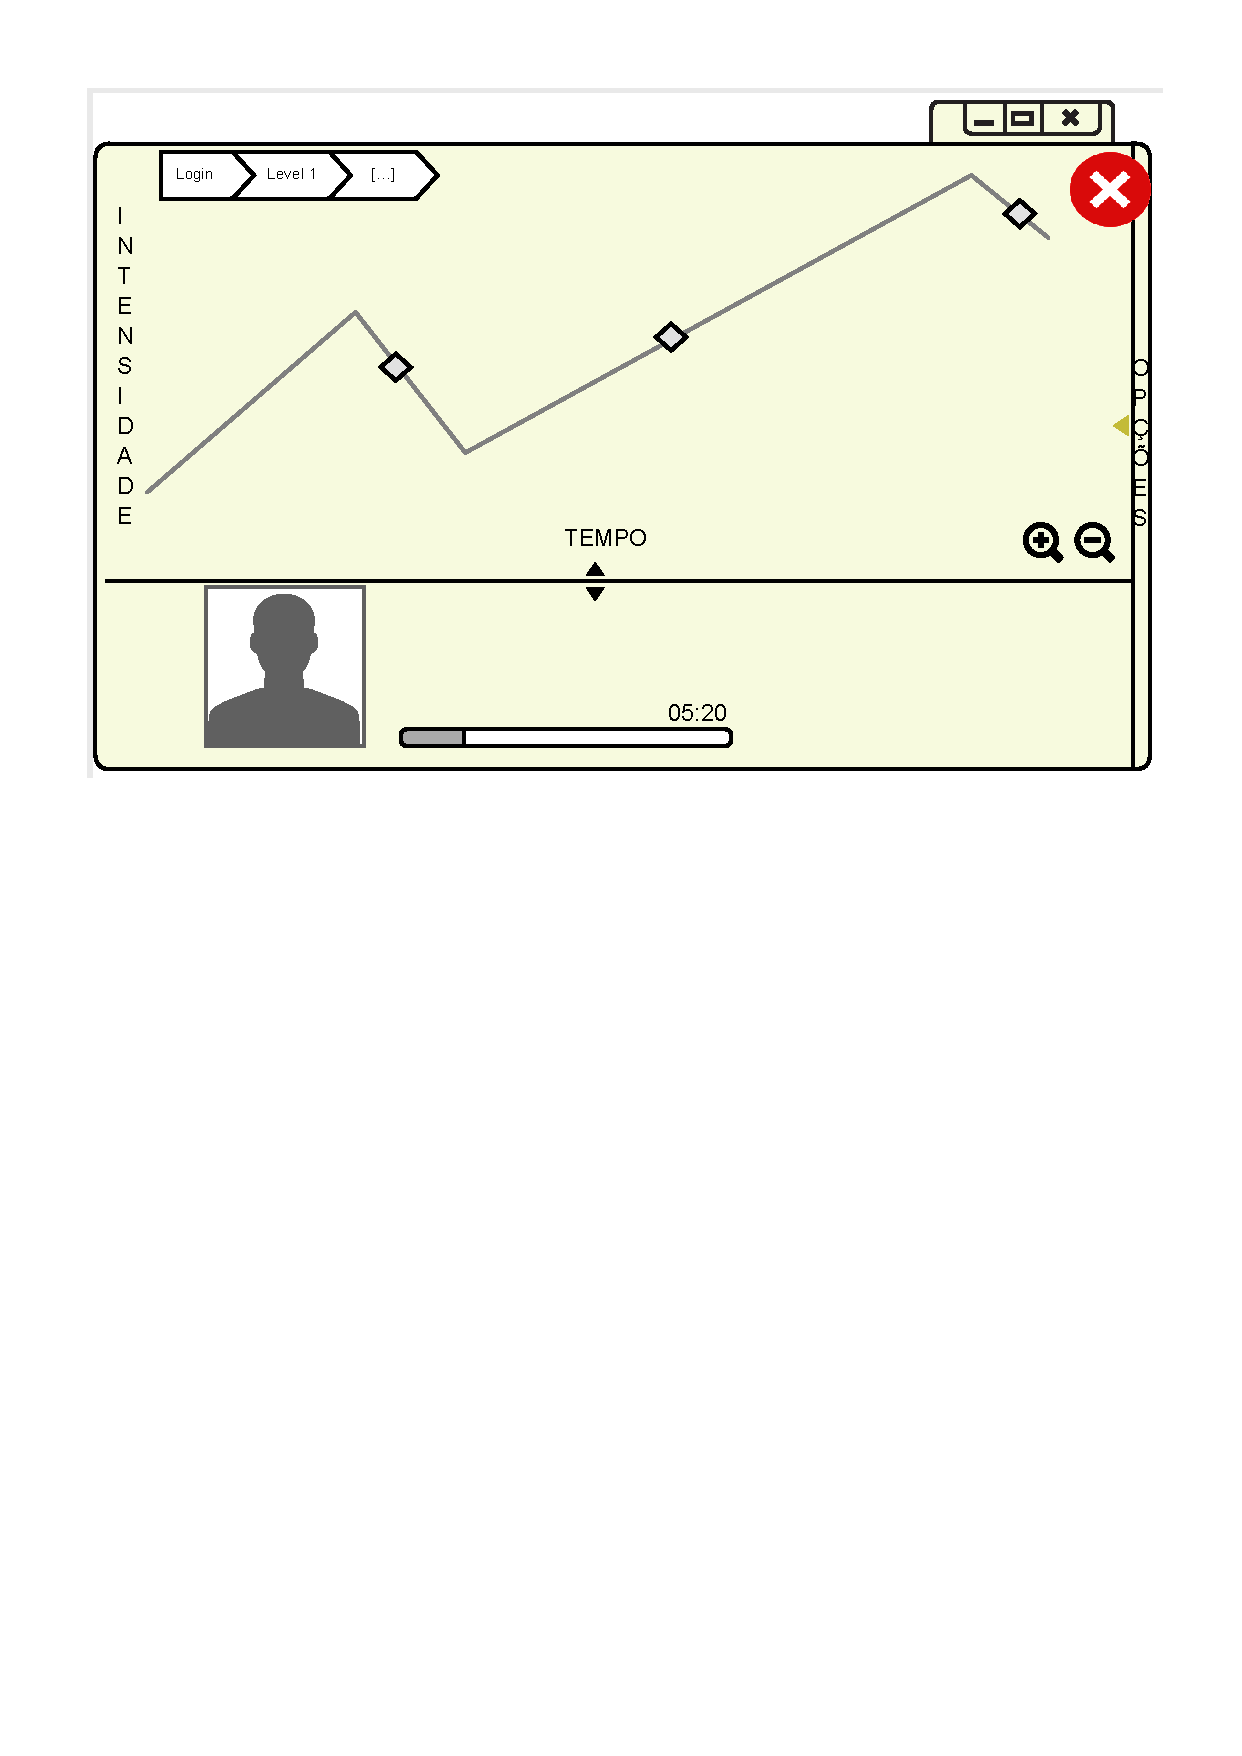
\includegraphics[scale=0.6]{imagens/2-3-1Analisar_Sessoes1.pdf}
\caption{Analise de Sessão}
\label{emotiv}
\end{figure}

\begin{figure}[h!]
\centering
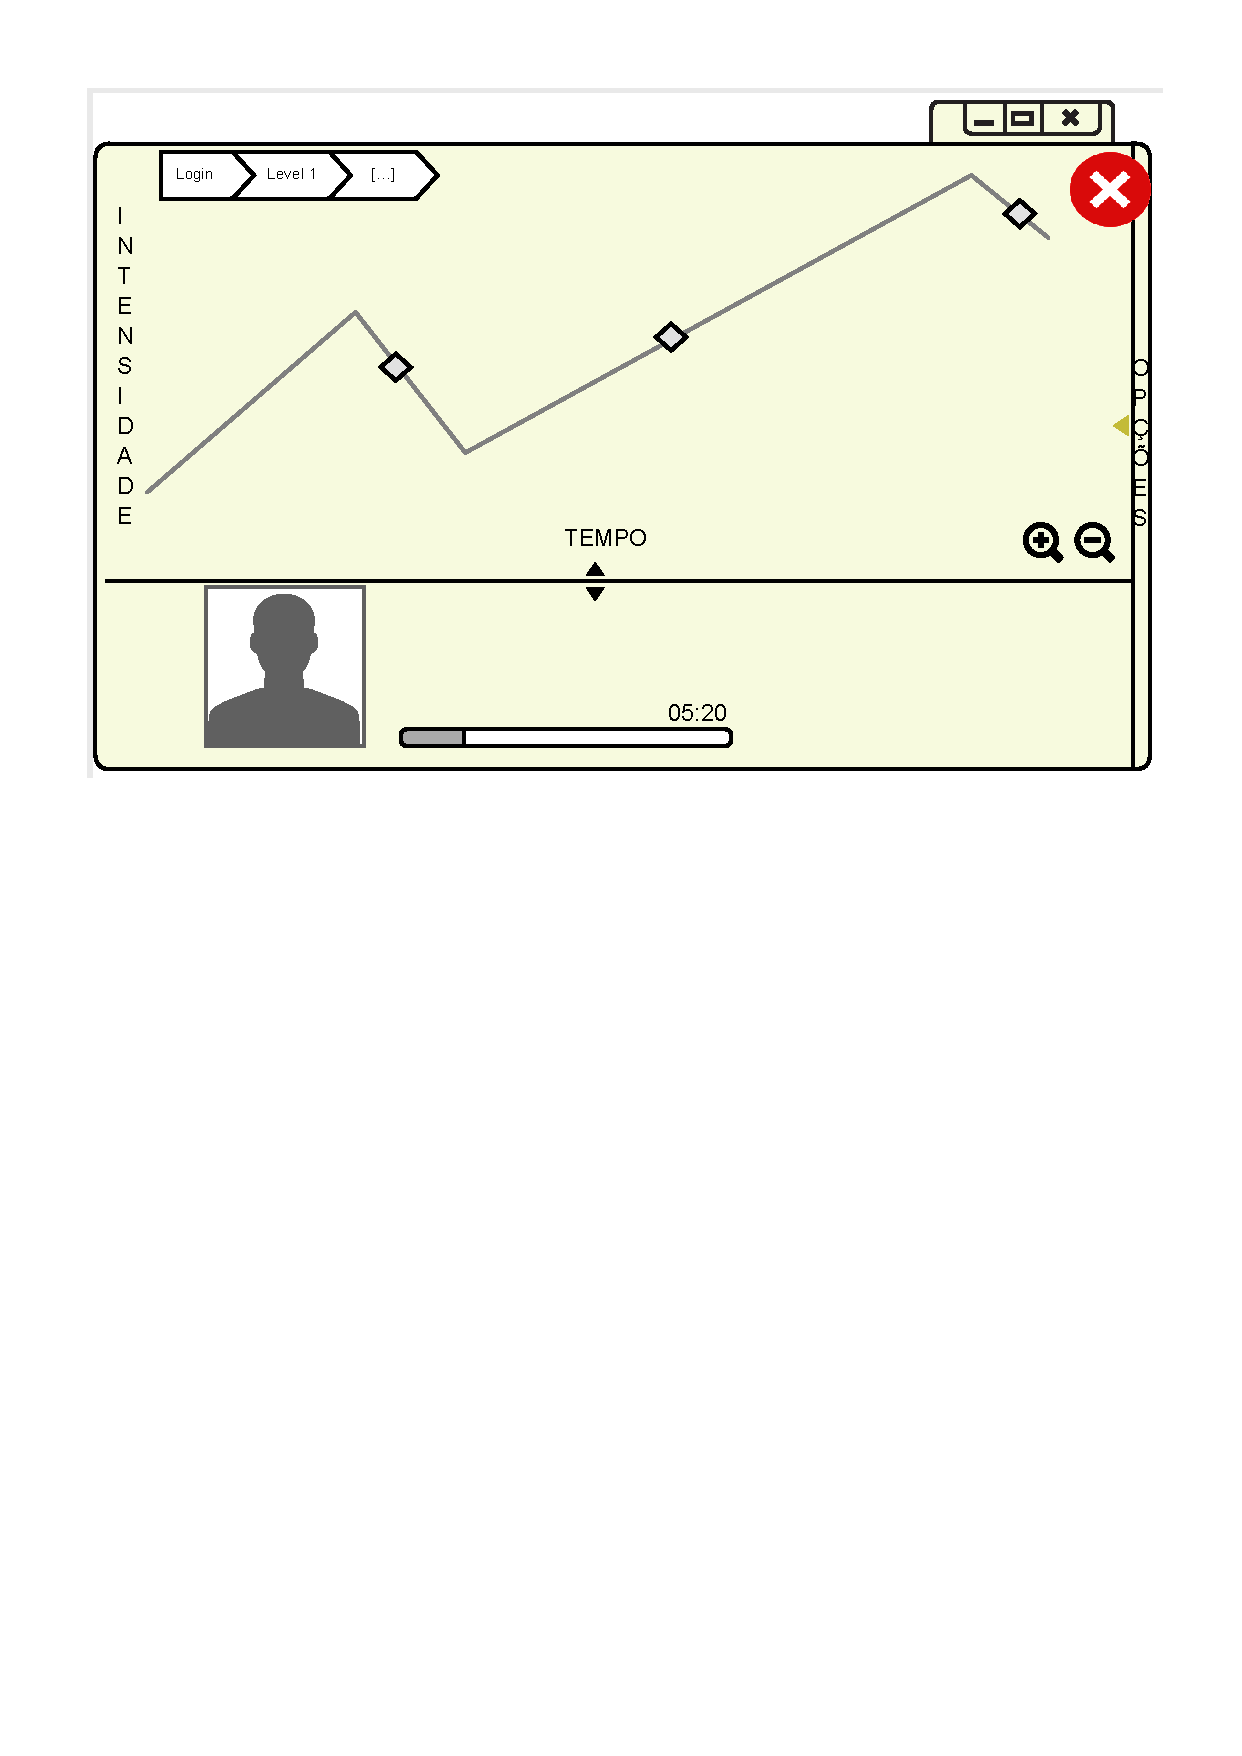
\includegraphics[scale=0.6]{imagens/2-3-1Analisar_Sessoes1.pdf}
\caption{Menu lateral expandido}
\label{emotiv1}
\end{figure}
\newpage

O Pequira conta também com uma opção para inserir notas nas fichas dos pacientes, embora esta funcionalidade não seja crítica ao sistema ela é útil para manter registro de detalhes importantes. nas Figuras \ref{alterar_ficha_cadastro}, \ref{alterar_ficha_notas} e \ref{alterar_ficha_notas_nova}, podemos ver como essas informações são adicionadas no sistema, bem como o cadstro de um paciente é atualizado.
A opção de cadastrar pacientes no menu inicial do sistema, Figura \ref{menu_sem_pendrive} leva a este mesmo conjunto de telas, com os dados não preenchidos. Note na Figura \ref{alterar_ficha_notas_nova} que é possivel estabelecer um link entre uma sessão de jogo e uma nota no sistema, muito embora o sistema ainda não conte com anexos de diferentes extensões como áudio ou pdf na ficha do paciente.

\begin{figure}[h]
\begin{subfigure}{0.5\textwidth}
\centering
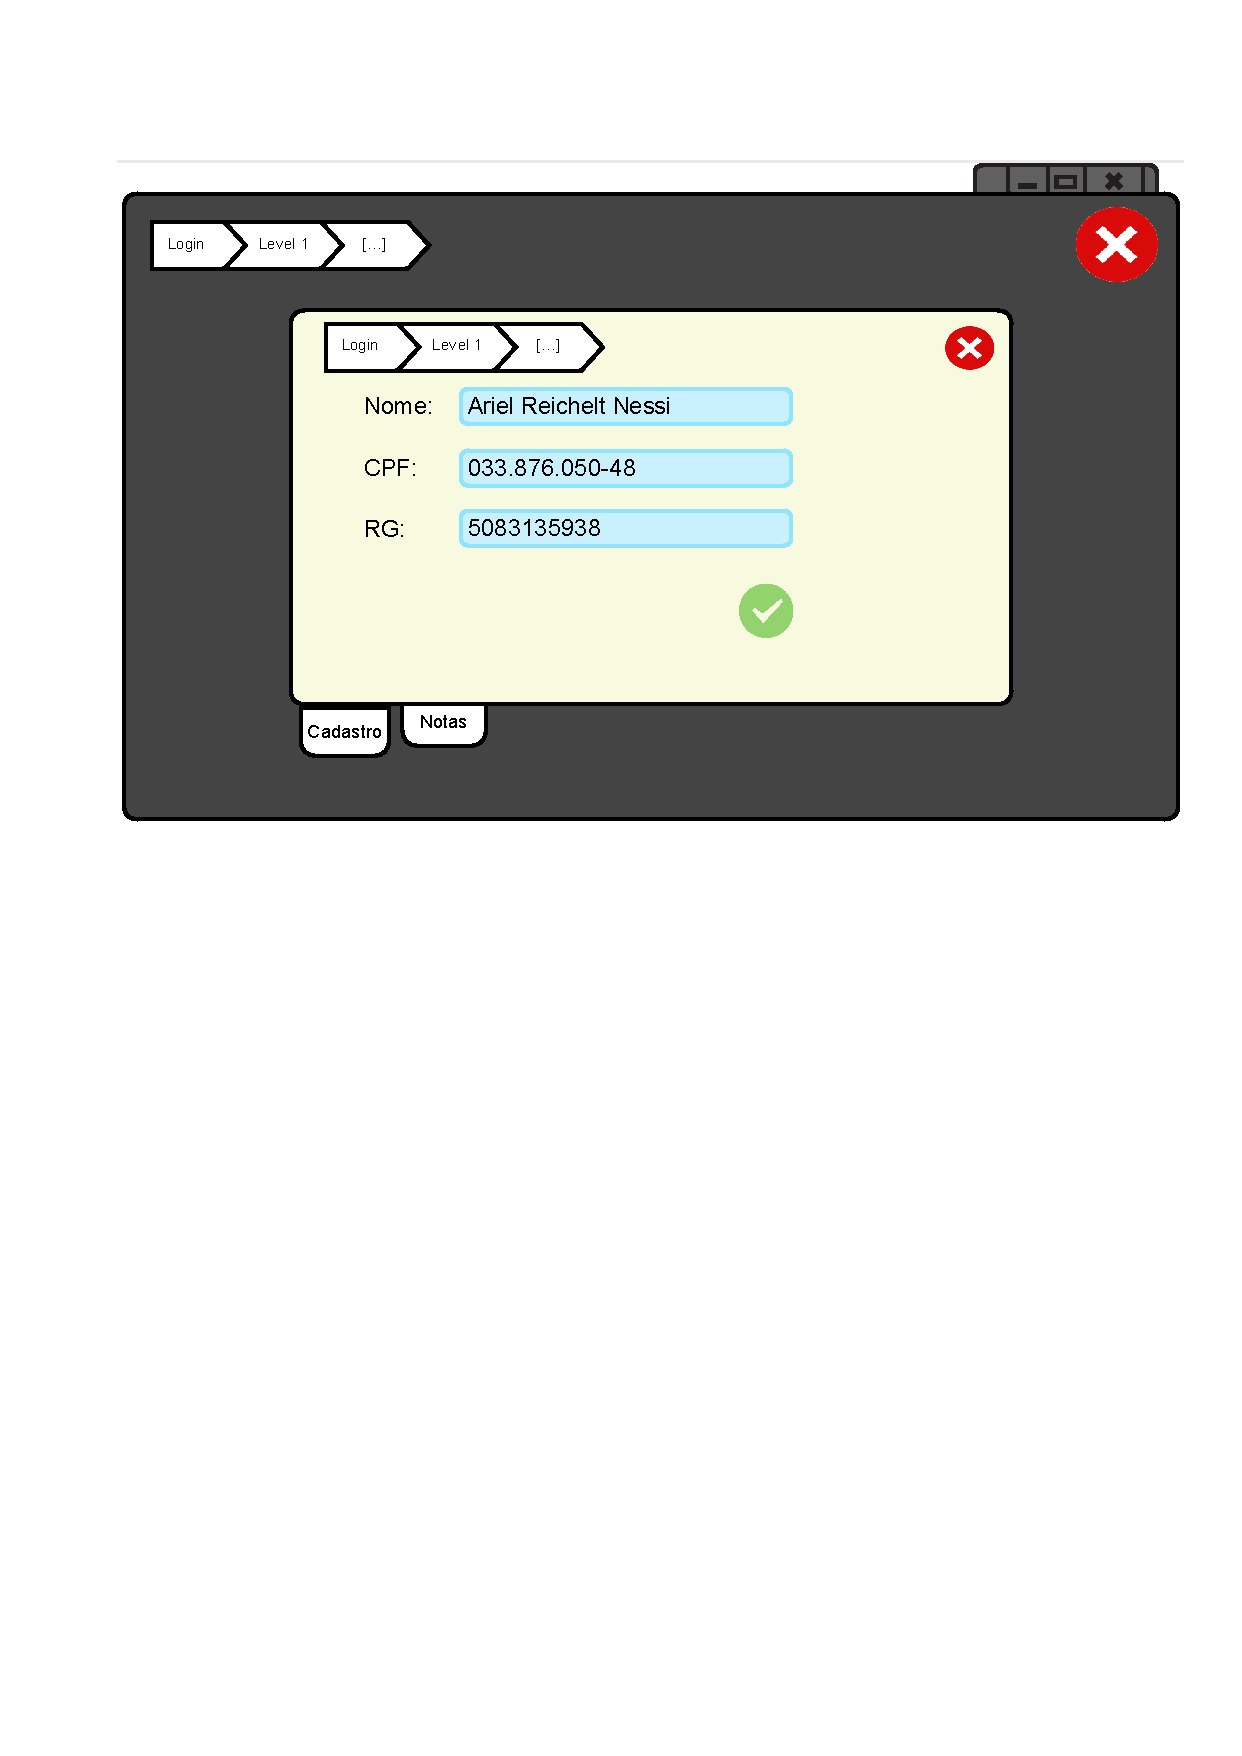
\includegraphics[scale=0.3]{imagens/Alterar_Ficha_Cadastro.pdf}
\caption{Alterando um Registro}
\label{alterar_ficha_cadastro}
\end{subfigure}
\begin{subfigure}{0.5\textwidth}
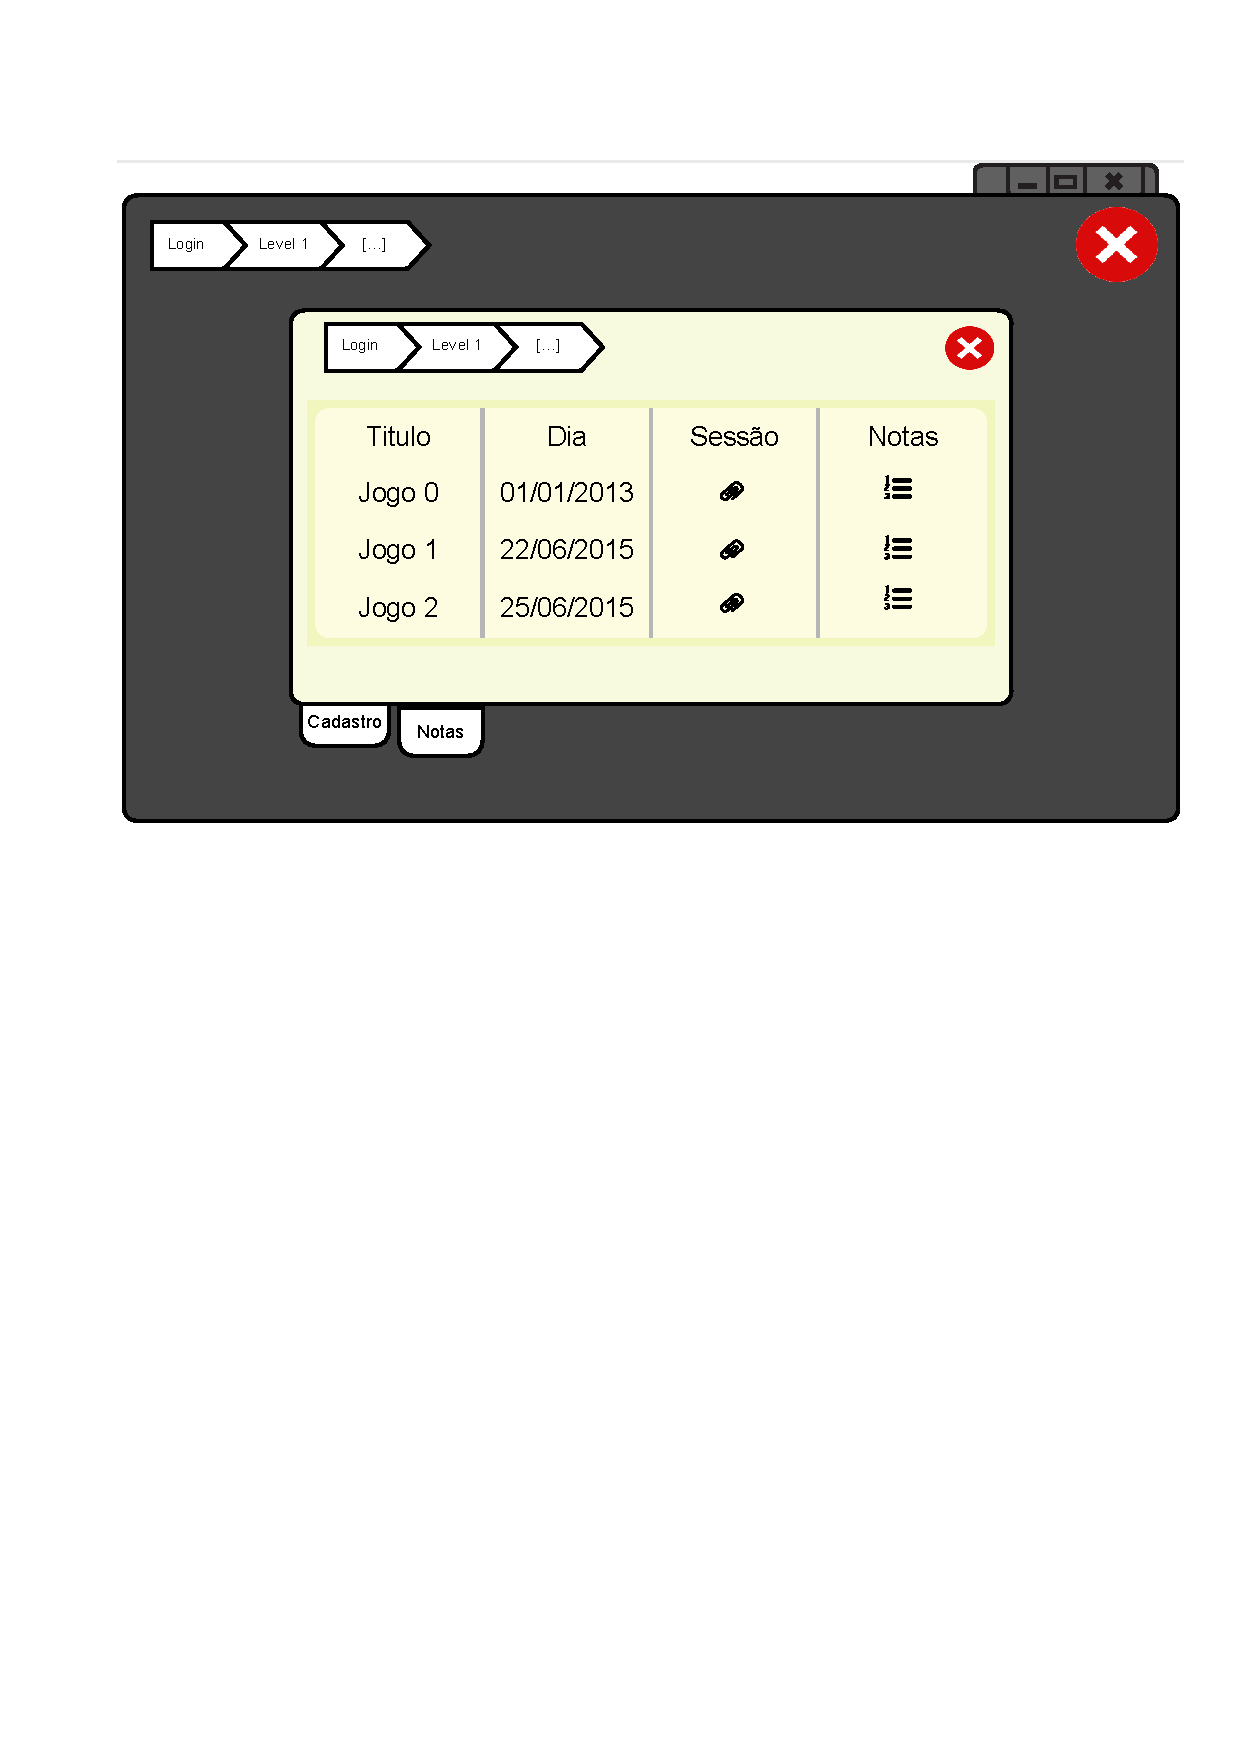
\includegraphics[scale=0.4]{imagens/Alterar_Ficha_Notas.pdf} 
\caption{Lista de notas sobre o paciente}
\label{alterar_ficha_notas}
\end{subfigure}
\end{figure}

\begin{figure}[h]
\centering
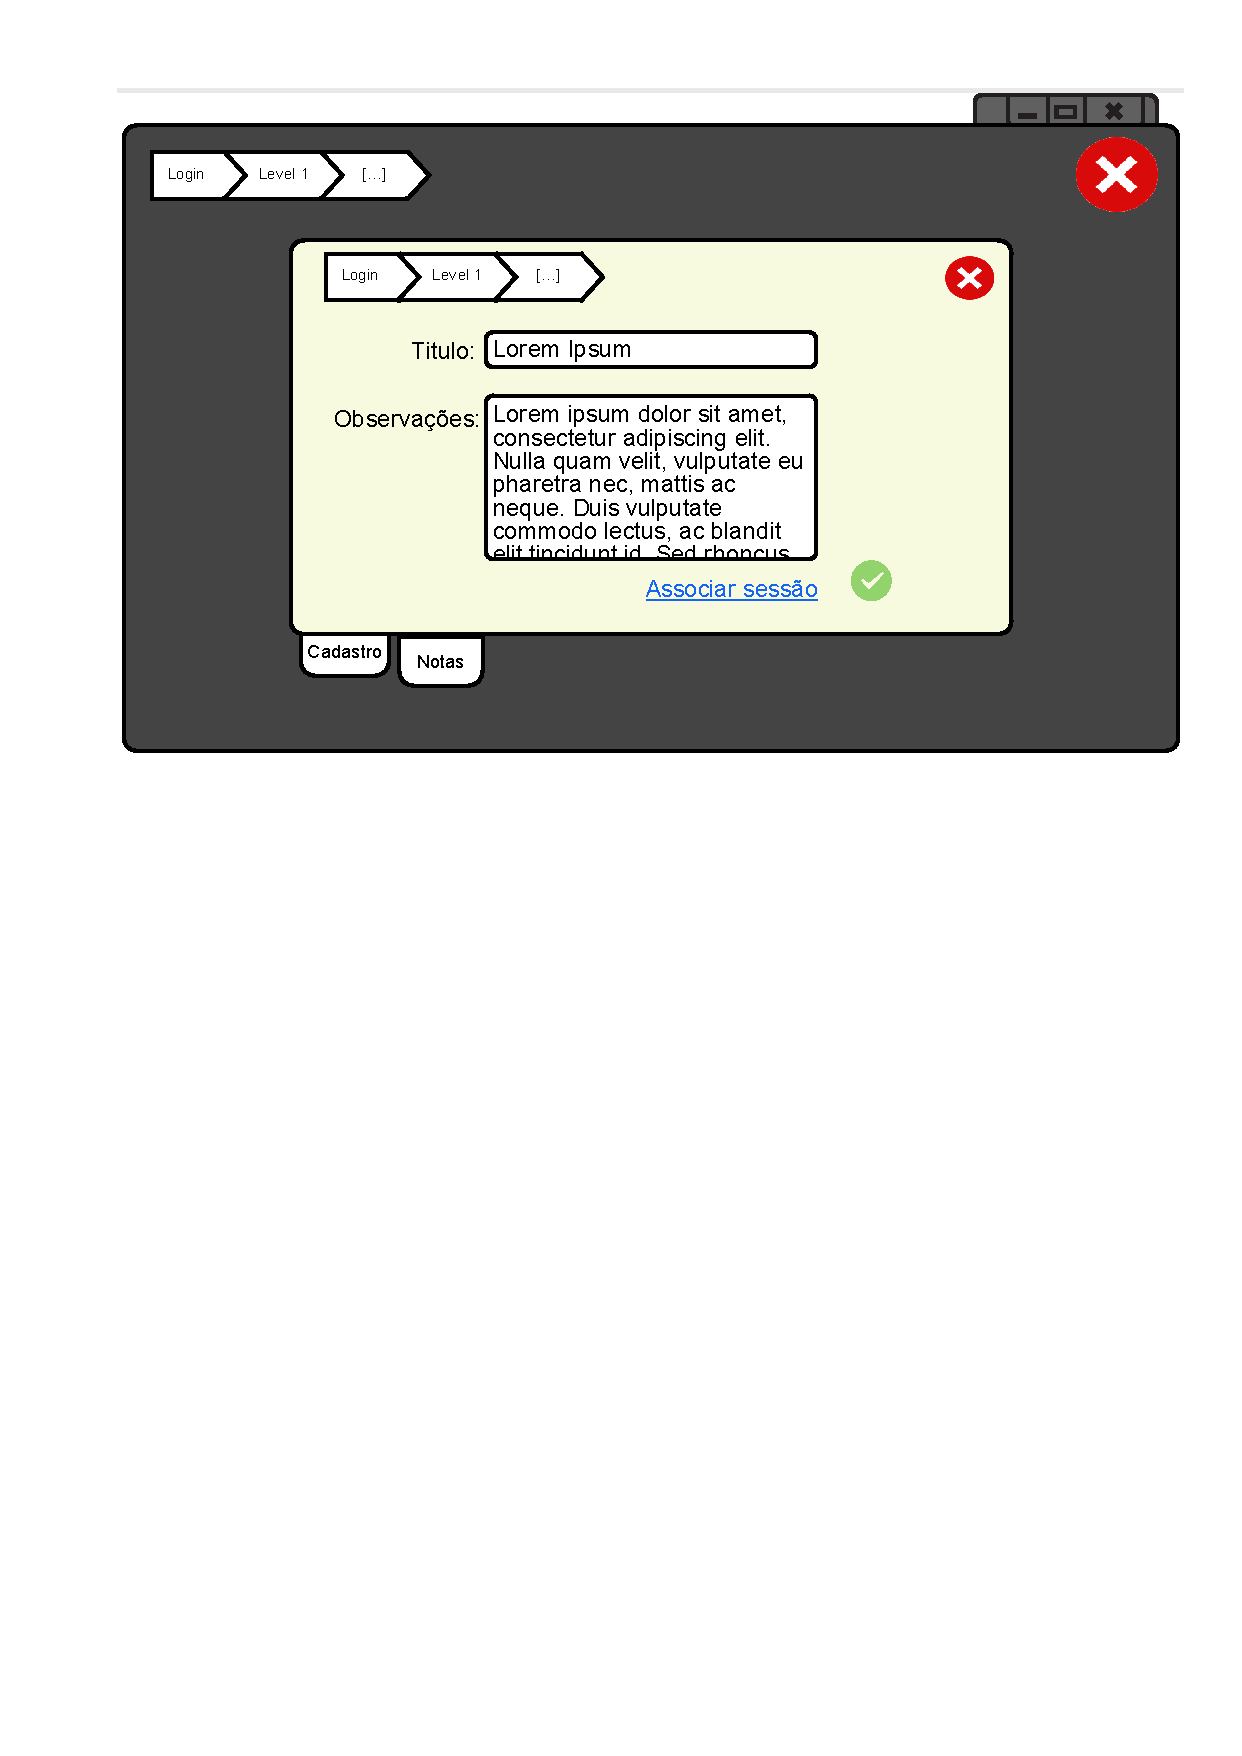
\includegraphics[scale=0.4]{imagens/Alterar_Ficha_Notas_Nova.pdf}
\caption{Inserindo uma nova anotação}
\label{alterar_ficha_notas_nova}
\end{figure}

\newpage{}
O Pequira na parte dos pacientes obriga a ser calibrado os equipamentos para a realização correta das atividades, temos a tela de calibragem pode ser vista na Figura \ref{calibragem}, na parte do emotiv temos uma informação para ajudar na calibragem vista na Figura \ref{instrucao_emotiv}, quando temos tudo pronto a tela da parte da calibragem fica verde como pode ser vista nas Figuras \ref{calibragem_emotiv}, \ref{calibragem_webcam}.

\begin{figure}[h]
\centering
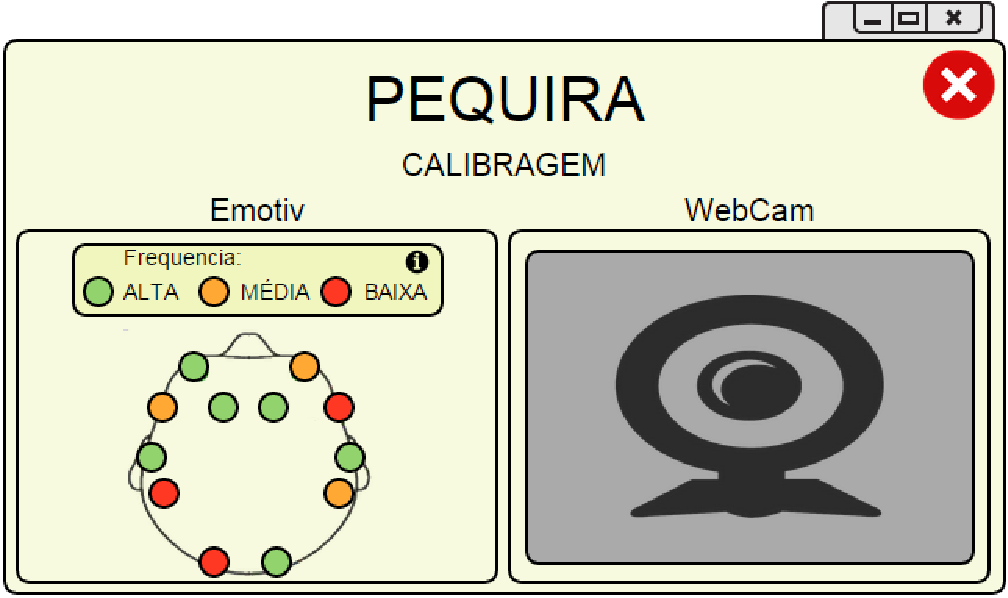
\includegraphics[scale=0.4]{imagens2/1-1Calibragem.pdf}
\caption{Calibragem dos equipamentos}
\label{calibragem}
\end{figure}

\begin{figure}[h]
\centering
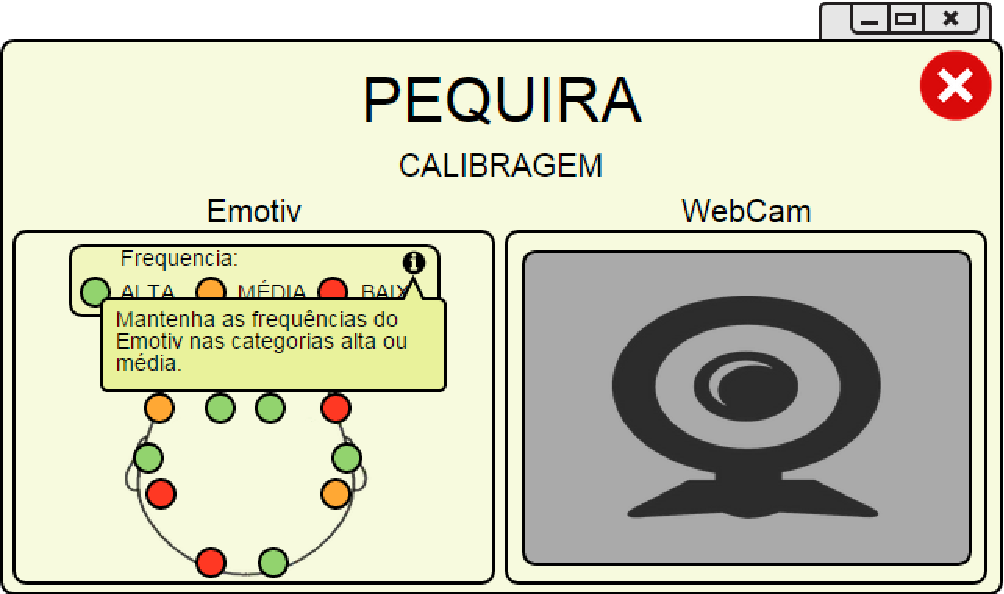
\includegraphics[scale=0.4]{imagens2/1-1-2Mensagemdeinstrucao.pdf}
\caption{Mensagem de Instrução do Emotiv}
\label{instrucao_emotiv}
\end{figure}

\begin{figure}[h]
\begin{subfigure}{0.5\textwidth}
\centering
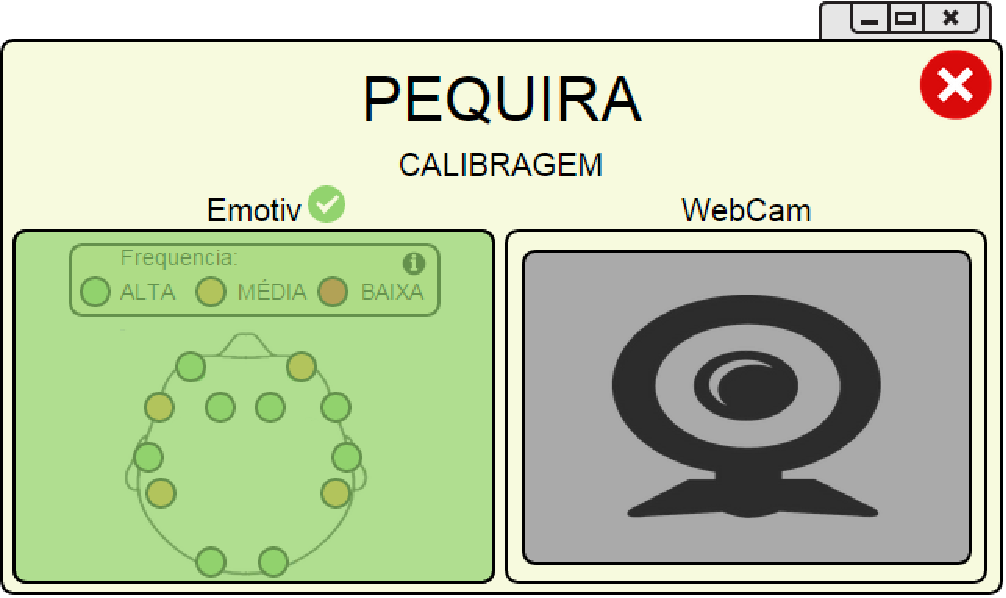
\includegraphics[scale=0.4]{imagens2/1-2CalibragemcompletaEmotiv.pdf}
\caption{Calibragem Completa do Emotiv}
\label{calibragem_emotiv}
\end{subfigure}
\begin{subfigure}{0.5\textwidth}
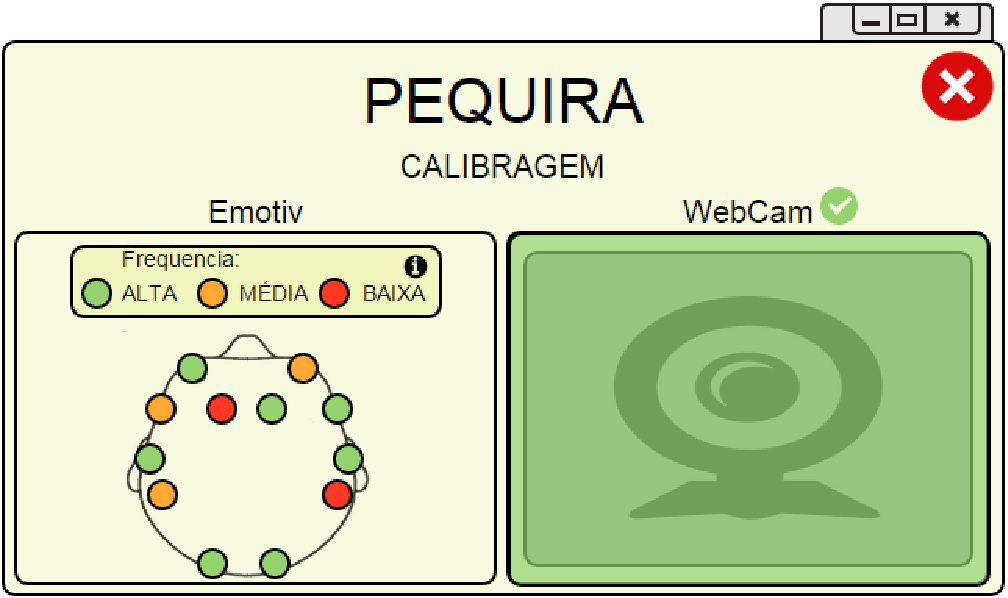
\includegraphics[scale=0.4]{imagens2/1-3CalibragemcompletaWebCam.pdf} 
\caption{Calibragem Completa da WebCam}
\label{calibragem_webcam}
\end{subfigure}
\end{figure}

\newpage{}
A tela das atividades podemos ver na Figura \ref{tela_das_atividades}, nela o paciente tem como pausar como mostra a Figura \ref{tela_atividades_pausada}, e também quando as atividades estão sendo carregadas temos apresentado na Figura \ref{tela_atividades_carregando}
\begin{figure}[h]
\centering
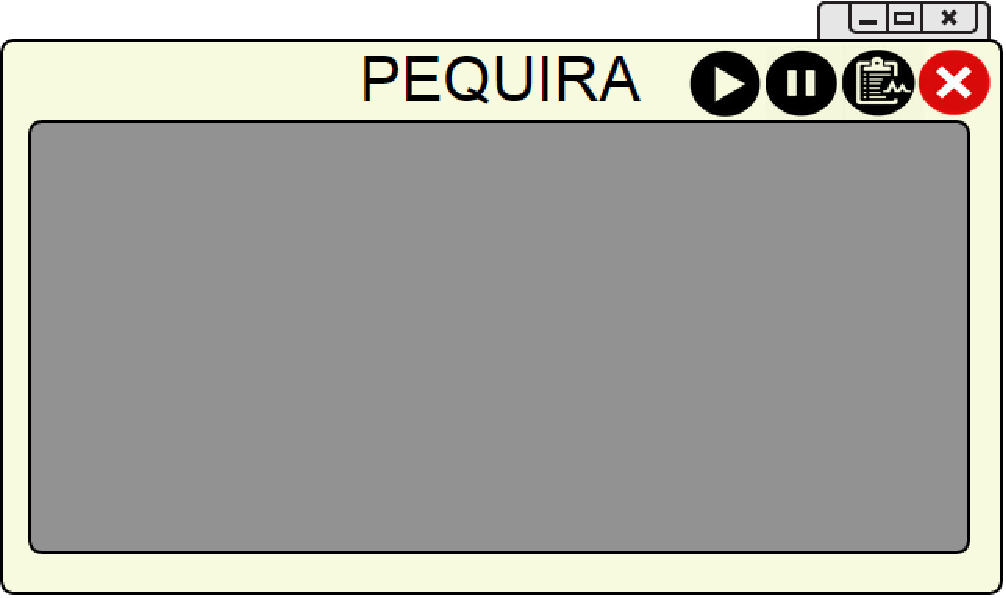
\includegraphics[scale=0.5]{imagens2/2-1TeladosJogos_Testes.pdf}
\caption{Tela das Atividades}
\label{tela_das_atividades}
\end{figure}

\begin{figure}[h]
\begin{subfigure}{0.5\textwidth}
\centering
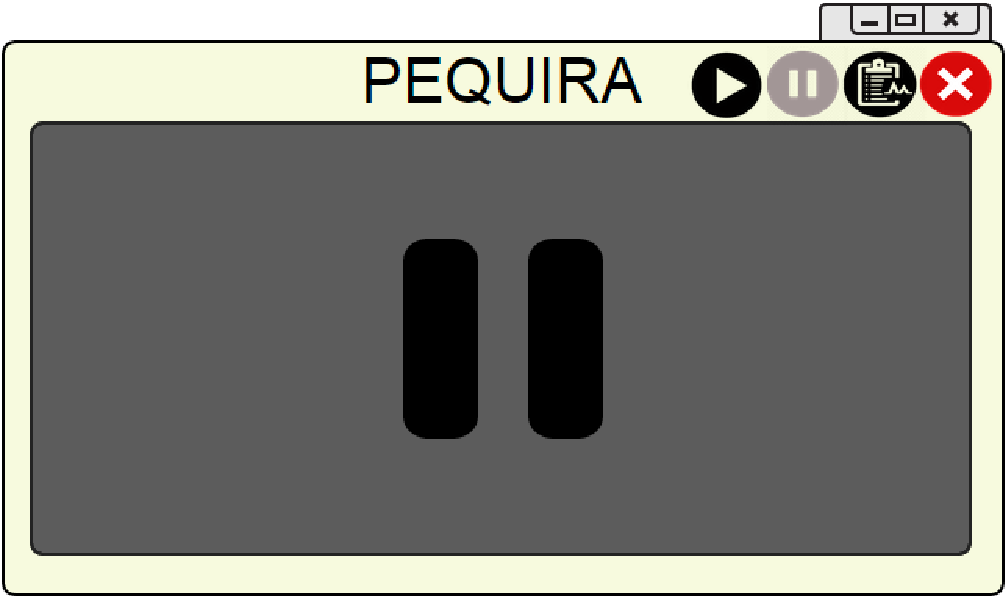
\includegraphics[scale=0.4]{imagens2/2-2TeladosJogosemPausado.pdf}
\caption{Tela das Atividades em Pause}
\label{tela_atividades_pausada}
\end{subfigure}
\begin{subfigure}{0.5\textwidth}
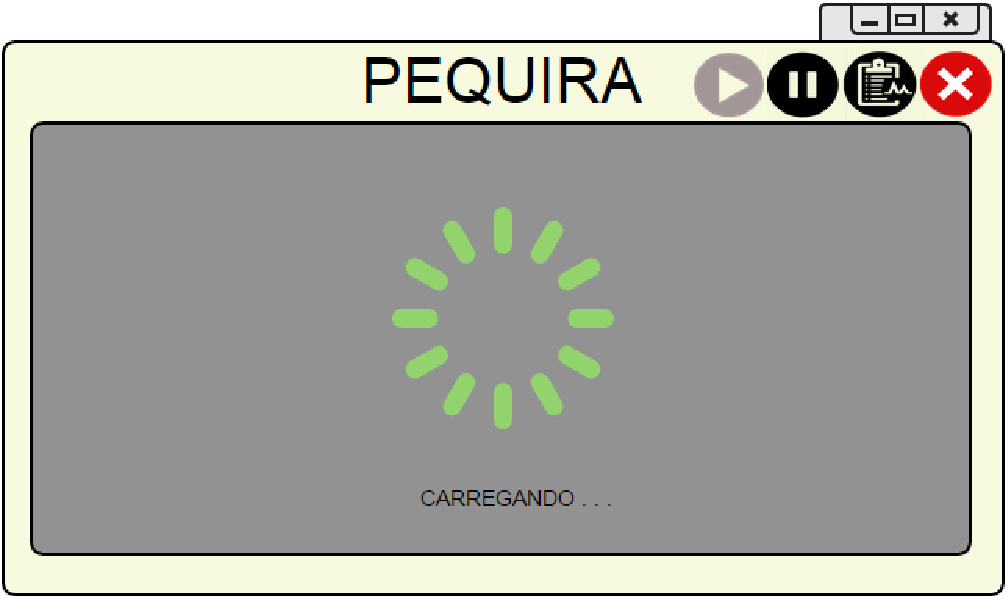
\includegraphics[scale=0.4]{imagens2/2-3Teladosjogos,playcarregandogame.pdf} 
\caption{Tela das Atividades Carregando}
\label{tela_atividades_carregando}
\end{subfigure}
\end{figure}
\newpage{}
O paciente ainda tem a possibilidade de ver o seu desempenho, quando estiver autorizado pelo medico, o desempenho é visto na Figura \ref{tela_de_desempenho}
\begin{figure}[h]
\centering
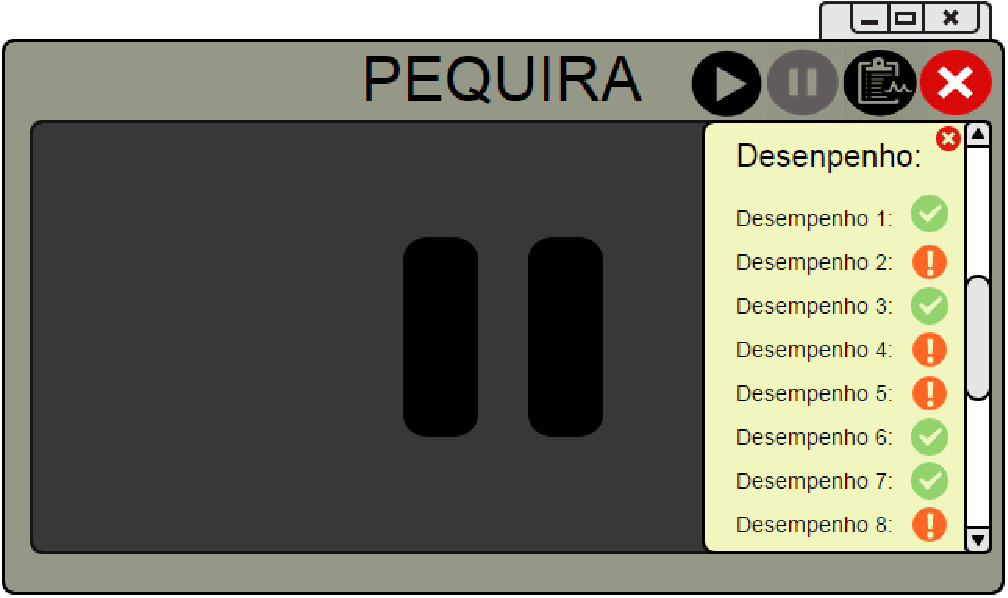
\includegraphics[scale=0.5]{imagens2/3-1TeladoDesempenho.pdf}
\caption{Tela do Desempenho}
\label{tela_de_desempenho}
\end{figure}

A tela de fechar o Pequira exige uma confirmação de saida, como pode ser visto na Figura \ref{fechar_pequira}

\begin{figure}[h]
\centering
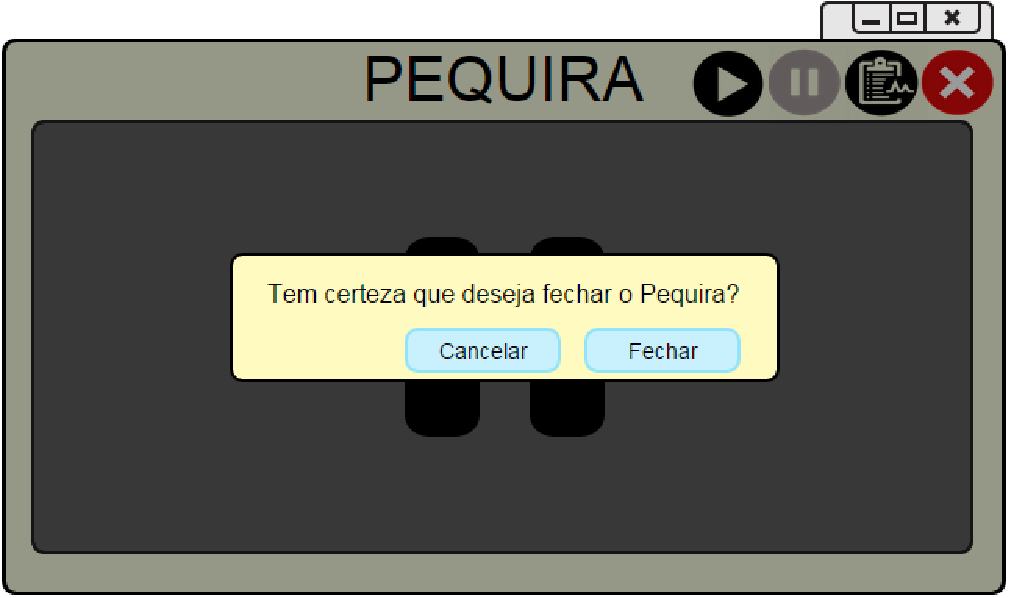
\includegraphics[scale=0.5]{imagens2/4-1FecharPequira.pdf}
\caption{Fechar Pequira}
\label{fechar_pequira}
\end{figure}

\section{Considerações Finais}
\paragraph{} Após a realização da modelagem a prototipação foi iniciada. A prototipação que visa demonstrar as telas propostas para o sistema explicando as funcionalidades de cada uma. Todo o sistema é feito para ser simples e de fácil uso. Através desse trabalho é possível avaliar a dificuldade de se produzir uma prototipação que condiz com a necessidade avaliada nas etapas anteriores seguindo uma padronização adequada.


\begin{thebibliography}{}                  
\bibitem{moqups} MOQUPS \textbf{https://moqups.com}.
\bibitem{emotiv} EMOTIV \textbf{https://emotiv.com/}.
\end{thebibliography}     
\end{document}
